\documentclass[tikz,border=10pt]{standalone}

\begin{document}

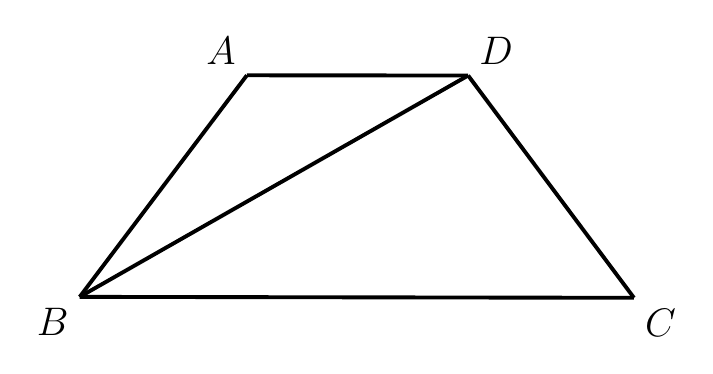
\begin{tikzpicture}[line join=round, line width=1.4pt, black]
\coordinate (A) at (-1.398,1.428);
\coordinate (B) at (-3.521,-1.386);
\coordinate (C) at (3.518,-1.398);
\coordinate (D) at (1.412,1.425);

  

  
  \draw (A) -- (B);
  \draw (A) -- (D);
  \draw (D) -- (C);
  \draw (B) -- (C);
  \draw (B) -- (D);

  
  \node[above left, font=\fontsize{14}{17}\selectfont\bfseries] at (A) {$A$};
  \node[above right, font=\fontsize{14}{17}\selectfont\bfseries] at (D) {$D$};
  \node[below left, font=\fontsize{14}{17}\selectfont\bfseries] at (B) {$B$};
  \node[below right, font=\fontsize{14}{17}\selectfont\bfseries] at (C) {$C$};
\end{tikzpicture}
\end{document}